\chapter{Теория}
\label{ch:intro}

Ряд Фурье — это способ представить периодическую функцию в виде суммы простых гармонических колебаний 
(синусов и косинусов) с разными частотами, амплитудами и фазами. \\

Функции $\{1, cos(x), sin(x), cos(2x), sin(2x) и т.д\}$ являются базисом пространтсва периодических функций (как в линейной алгебре
есть базис, допустим, трехмерного пространтсва, который состоит из ортов i, j и k, и все вектора в этом пространстве могут быть
разложены по этим ортам, т.е представлены в виде их линеной комбинации), поэтому почти любую периодическую функцию можно представить
в виде суммы функций, принадлежащих этому базису. \\

Еще одним примером разложения является ряд Тейлора. Базисом для пространства функций является множество функций $\{1, x, x^2, x^3, \dots\}$,
по которому также можно разложить почти любую функцию, т.е. представить в виде линейной комбинации многочленов.

Ряд Фурье и его коэффициенты вычисляются следующим образом:

\begin{figure}[H]
    \centering
    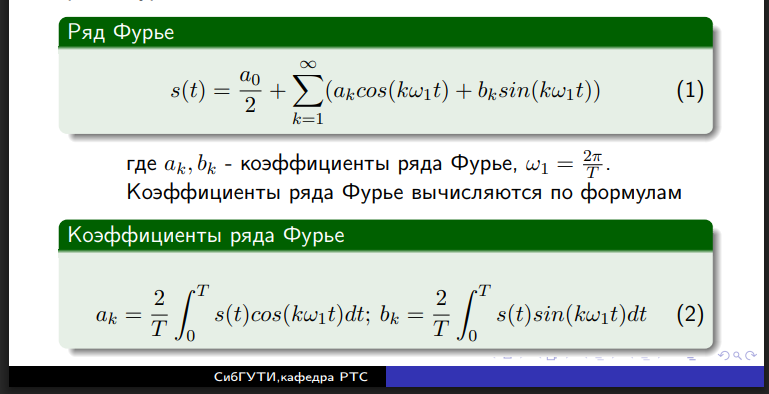
\includegraphics[width=1.0\textwidth]{furie_formula.png}
    \caption{Формула ряда Фурье и коэффициентов}
\end{figure}

где $\frac{a_0}{2}$ "--- постоянная составляющая (или среднее значение сигнала), \\
$a_k$ и $b_k$ "--- коэффициенты ряда Фурье, $a_k$ отвечает за амплитуды чётных (симметричных) составляющих функции
и показывают, насколько сильно в сигнале выражена компонента вида cos($\omega_0t$), а $b_k$ отвечает за амплитуды нечётных (асимметричных) составляющих функции
и показывают, насколько сильно в сигнале выражена компонента вида sin($\omega_0t$). \\
$k$ "--- номер гармоники ($k = 1,2,3,4,\dots$), \\
$\cos(k\omega_1 t)$ и $\sin(k\omega_1 t)$ "--- базисные функции.

Важно заметить, что сигнал, который нужно разложить в ряд Фурье, должен содержать только гармонники с частотой кратной $w_1$. Если
такое условие не выполняется, то сигнал не будет периодическим и разложить его в классический ряд Фурье невозможно.

Пример вычисления коэффициентов ряда Фурье:

\begin{figure}[H]
    \centering
    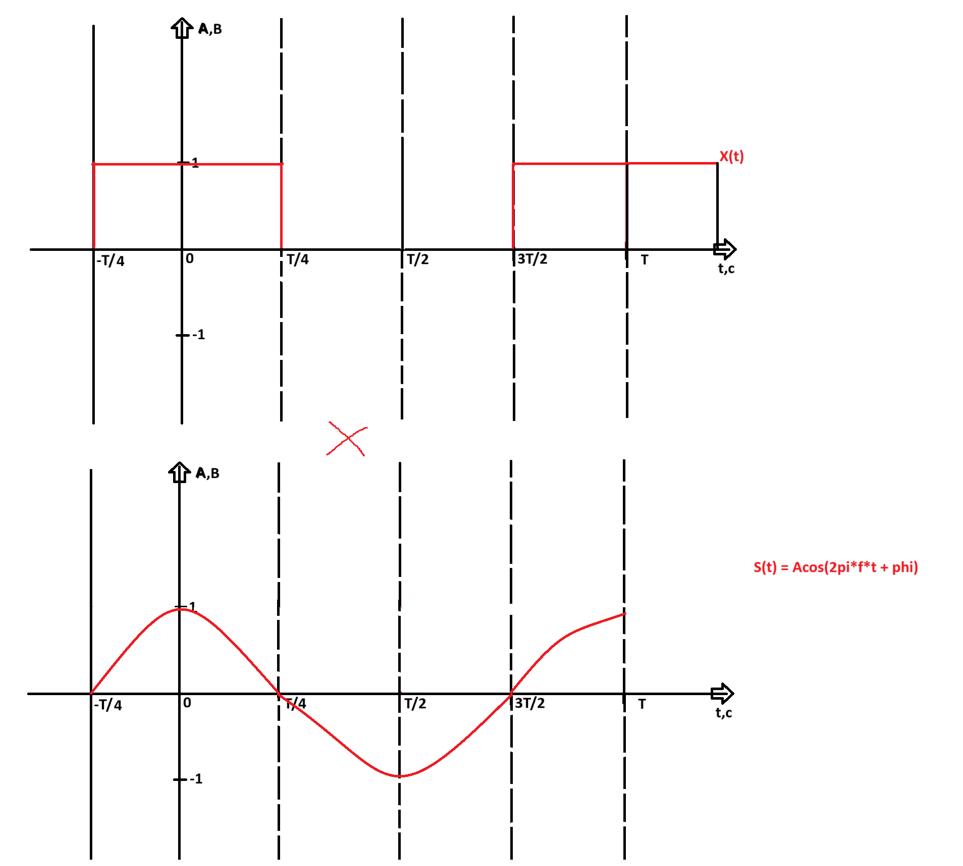
\includegraphics[width=1.0\textwidth]{a_comp_1.png}
    \caption{Геометрическая интерпретация вычисления $a_k$}
\end{figure}


\begin{figure}[H]
    \centering
    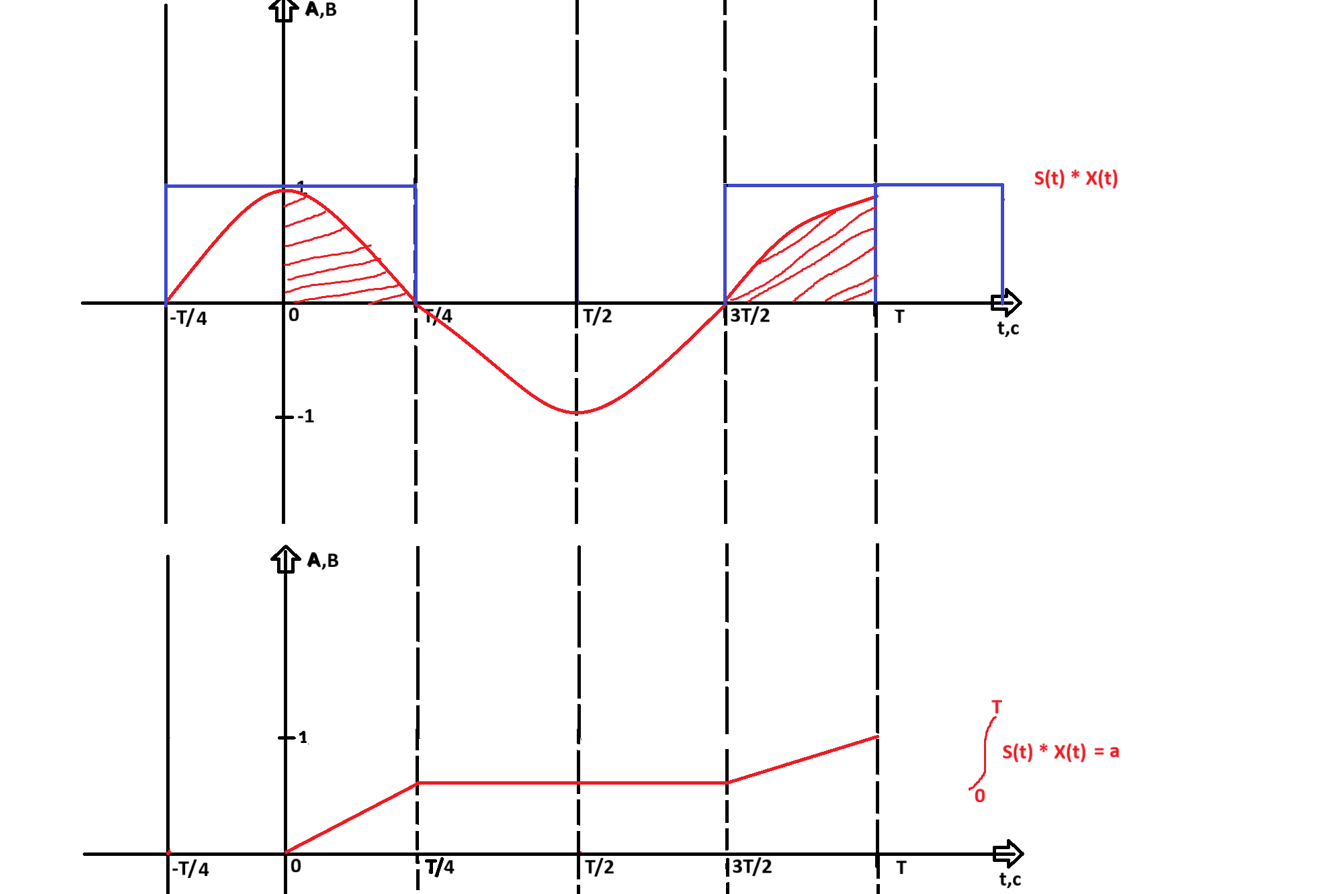
\includegraphics[width=1.0\textwidth]{a_comp_2.png}
    \caption{Геометрическая интерпретация вычисления $a_k$}
\end{figure}

\begin{figure}[H]
    \centering
    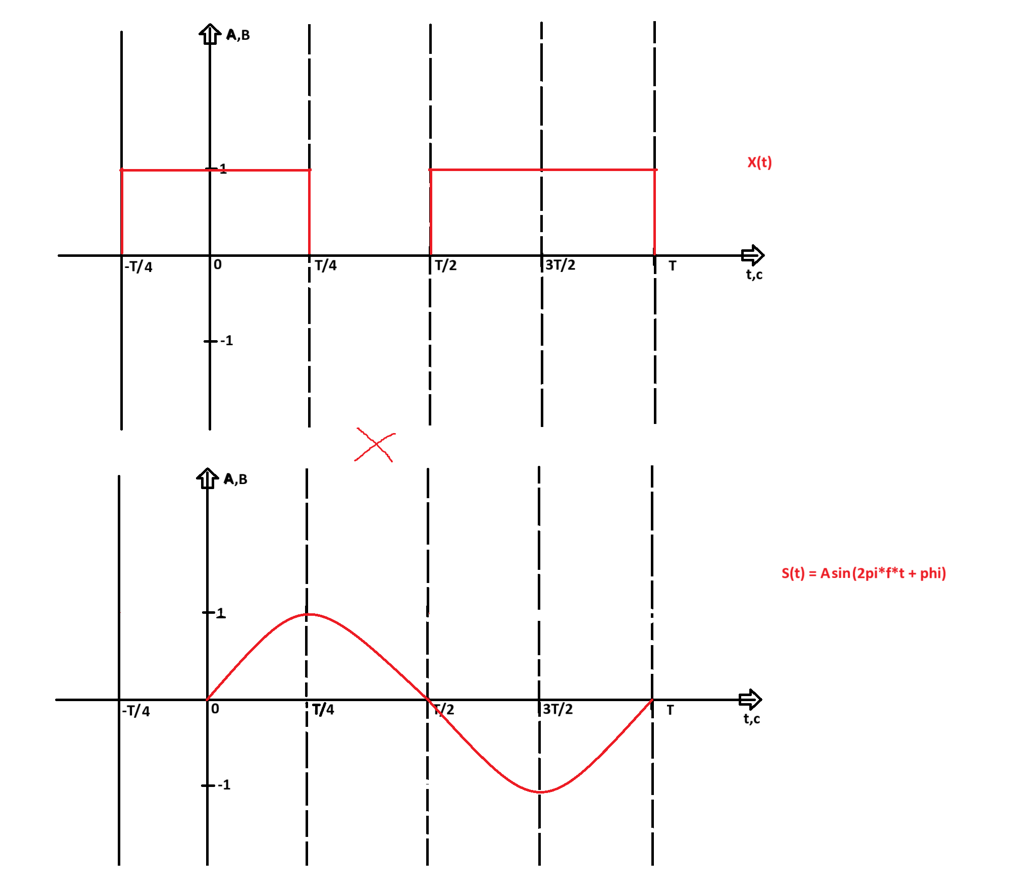
\includegraphics[width=1.0\textwidth]{b_comp_1.png}
    \caption{Геометрическая интерпретация вычисления $b_k$}
\end{figure}


\begin{figure}[H]
    \centering
    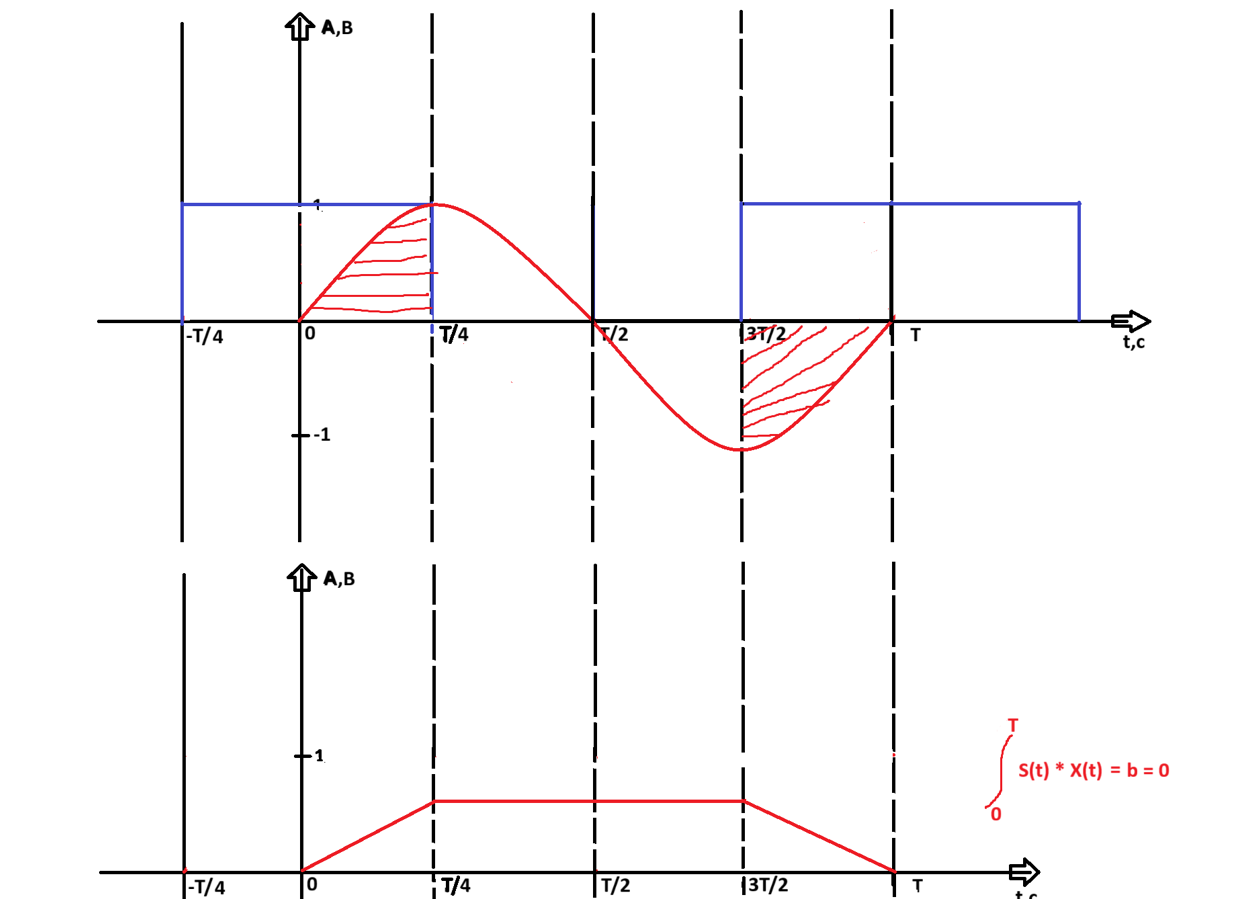
\includegraphics[width=1.0\textwidth]{b_comp_2.png}
    \caption{Геометрическая интерпретация вычисления $b_k$}
\end{figure}

Заметим, что исходный сигнал (прямоугольный) - четный, поэтому коэффциенты $b_k$ будут всегда равны нулю и в разложении
будет участвовать только cos($\omega_0t$).

\subsection*{\textbf{Пример}}

Рассмотрим простейший сигнал $cos(2\pi*t)$. Рассчитаем для него $a_1$ и $b_1$: \\

Перемножим наш сигнал на cos-компоненту при k = 1

\begin{figure}[H]
    \centering
    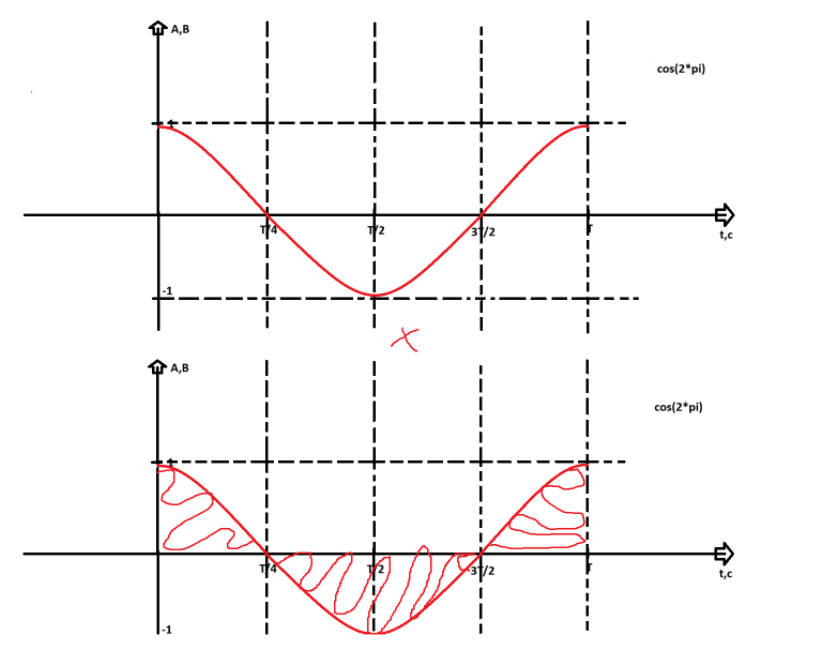
\includegraphics[width=1.0\textwidth]{ex_mul.png}
    \caption{Вычисление $a_1$}
\end{figure}

То, как будет изменяться интеграл от их произведения
\begin{figure}[H]
    \centering
    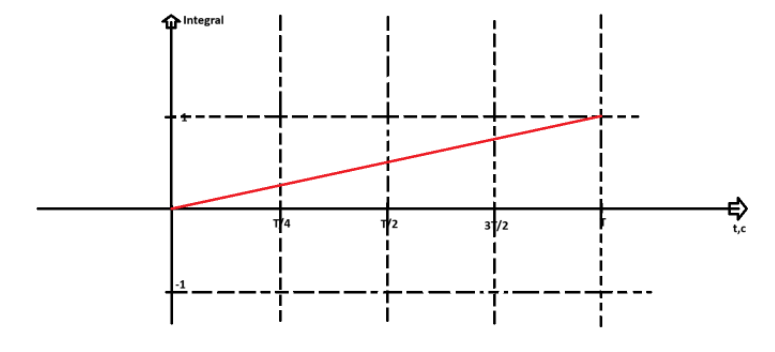
\includegraphics[width=1.0\textwidth]{ex_int1.png}
    \caption{Вычисление $a_1$}
\end{figure}

Значение интеграла в момент времени T будет равно $\pi$, это значит, что в нашем
сигнале присутствует cos-компонента с частотой 1Гц (что логично). \\

Теперь рассчитаем $b_1$, т.е сколько в нашем сигнале содержится компоненты $sin(2\pi*t)$

\begin{figure}[H]
    \centering
    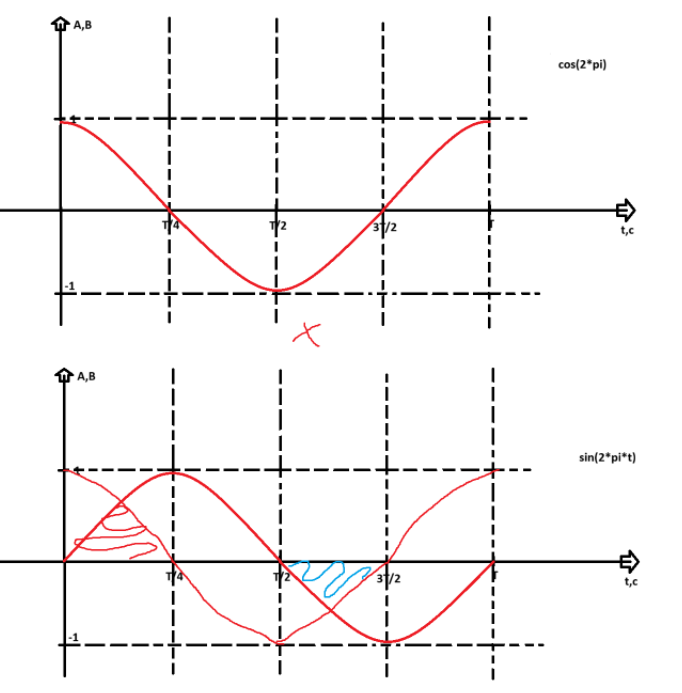
\includegraphics[width=1.0\textwidth]{ex_mul_2.png}
    \caption{Вычисление $a_1$}
\end{figure}

То, как будет изменяться интеграл от их произведения
\begin{figure}[H]
    \centering
    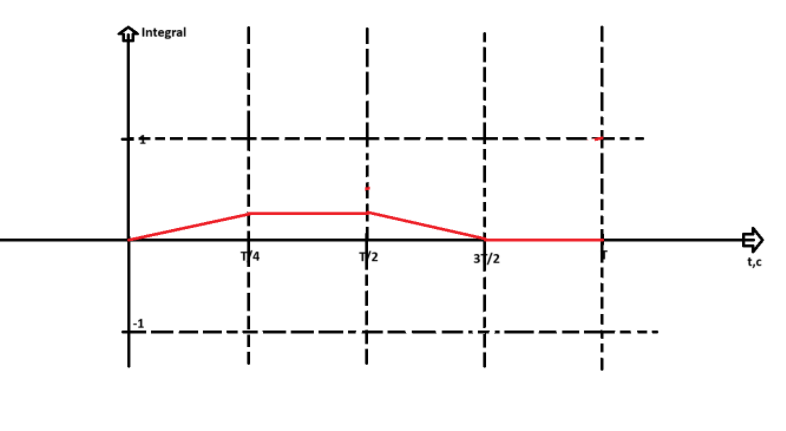
\includegraphics[width=1.0\textwidth]{int2.png}
    \caption{Вычисление $a_1$}
\end{figure}

Значение интеграла в момент времени T будет равно 0, это значит, что в нашем
сигнале не присутствует sin-компонента с частотой 1Гц (что логично, ведь наш сигнал изначально косинус, который симметричен). \\

В нашем сигнале точно нет никаких sin-компонент. Может, есть компонента $cos(4\pi*t)$?


\begin{figure}[H]
    \centering
    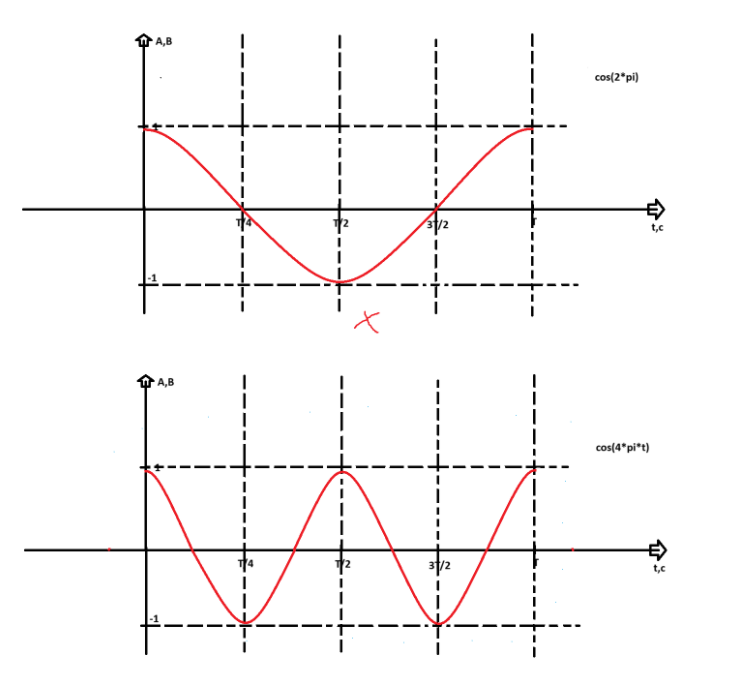
\includegraphics[width=1.0\textwidth]{ex_mul2.png}
    \caption{Вычисление $a_1$}
\end{figure}

То, как будет изменяться интеграл от их произведения
\begin{figure}[H]
    \centering
    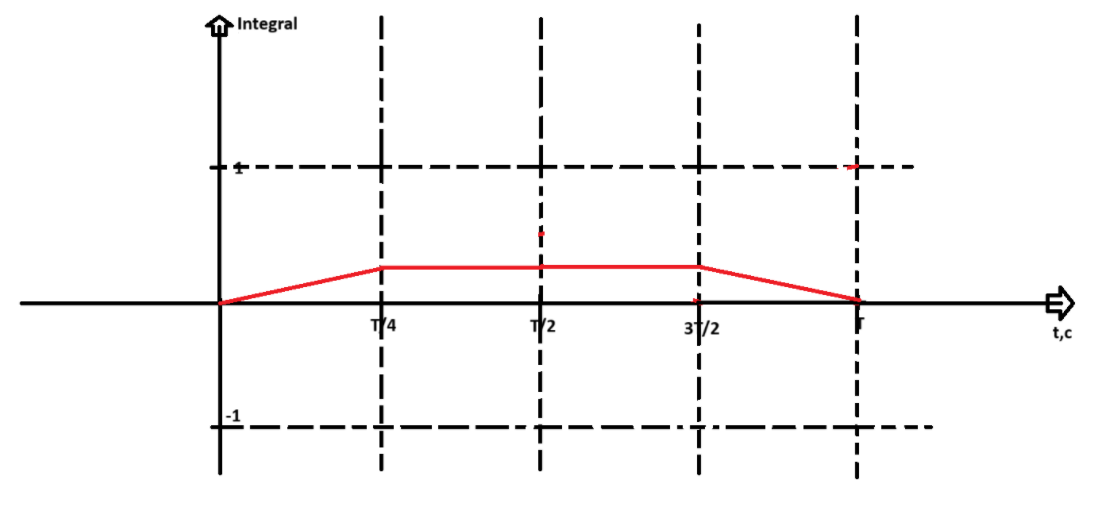
\includegraphics[width=1.0\textwidth]{int3.png}
    \caption{Вычисление $a_1$}
\end{figure}

В графике много симметричностей, которые по итогу дают ноль. При увеличении частоты компонент ничего не поменяется: будут симетричности,
которые в сумме будут сводить интеграл к нулю. Это значит, что в нашем сигнале только 1 компонента $cos(2\pi*t)$. \\

\subsection*{\textbf{Иная форма записи ряда Фурье}}

Классическая форма ряда Фурье не очень удобна для вычисления, поэтому ее заменяют косинусной формой ряда Фурье:

$$\frac{A_0}{2}+\sum_{n=1}^{\inf}A_n*cos(n*\omega_1t+\phi_n)$$

где $A_n = \sqrt{a_n^2+b_n^2}$, а $\phi_n = -arctg(\frac{b_n}{a_n})$

\subsection*{\textbf{Прямоугольный сигнал и ряд Фурье для него}}

Прямоугольный сигнал имеет следующие характеристики: \\

$T(s)$ - период (время одного колебания) \\
$\tau(s)$ - длительность сигнала (то время, когда сигнал не равен 0) \\
$A (B)$ - максимальное значение сигнала \\
$D = \frac{\tau}{T}$ - коэффициент заполнения (показывает какую долю периода занимает импульс) \\

Разложение в ряд Фурье для прямоугольного нечетного сигнала выглядит следующим образом:


\begin{figure}[H]
    \centering
    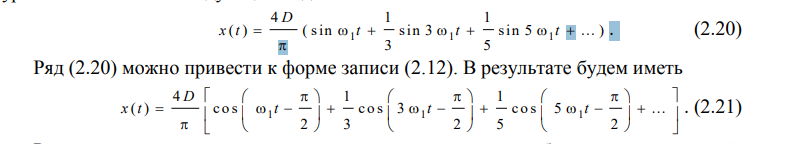
\includegraphics[width=1.0\textwidth]{rect_async_formul.png}
    \caption{Формула для нечетного прямоугольного сигнала}
\end{figure}

Видим, что в таком разложении только sin компоненты, причем при четных n sin=0, поэтому их исключаем.

Если сигнал четный, то формула будет следующей

\begin{figure}[H]
    \centering
    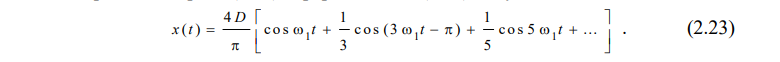
\includegraphics[width=1.0\textwidth]{rect_sync_formula.png}
    \caption{Формула для четного прямоугольного сигнала}
\end{figure}

Здесь уже только cos компоненты

\subsection*{\textbf{Ортогональность сигнала}}

Два сигнала \(x(t)\) и \(y(t)\) называются \textbf{ортогональными} на интервале \([a, b]\), если их скалярное произведение равно нулю:

\[
\langle x, y \rangle = \int_{a}^{b} x(t) \, y(t) \, dt = 0
\]

Это означает, что сигналы в радиоканале "не мешают" друг другу, т.е не заглушают друг друга их их можно передавать вместе. Эта идея используется в таких
технологиях, как CDMA и OFDM.
\endinput